\documentclass[11pt,a4paper]{article}
\usepackage[utf8]{inputenc}
\usepackage[T1]{fontenc}
\usepackage[french]{babel}
\usepackage{amsmath}
\usepackage{amssymb}
\usepackage{graphicx}
\usepackage[left=3cm,right=3cm,top=3cm,bottom=3cm]{geometry}

\title{\textbf{\huge{Rapport Programmation Avancée \& Projet} \\[1cm]Équation de Black et Scholes\\[1cm]}}
\author{\textbf{\Large{Adib HABBOU - Alae KHIDOUR}}}
\date{}

\usepackage{titling}
\renewcommand\maketitlehooka{\null\mbox{}\vfill}
\renewcommand\maketitlehookd{\vfill\null}

\begin{document}

\begin{titlingpage}
\maketitle
\end{titlingpage}
\newpage

\tableofcontents
\newpage

\section{Étude théorique}

\subsection{Équation de Black et Scholes}

Le modèle de Black et Scholes est basé sur l'hypothèse que les marchés financiers sont efficients et que les prix des actifs reflètent toutes les informations disponibles sur ces actifs. Selon cette hypothèse, il est impossible pour un investisseur de réaliser des profits à long terme en agissant sur le marché, à moins de prendre des risques supplémentaires.\\

Le modèle de Black et Scholes utilise également l'hypothèse que les taux d'intérêt sans risque sont constants et connus à l'avance. Il suppose également que la volatilité de l'actif sous-jacent est constante et connue à l'avance (la volatilité mesure la fluctuation des prix de l'actif sous-jacent).\\

En résumé, le modèle de Black et Scholes est un modèle mathématique utilisé pour déterminer le prix d'une option en prenant en compte les taux d'intérêt sans risque, la volatilité de l'actif sous-jacent et la date d'expiration de l'option. Il a été largement utilisé dans l'industrie financière pour la tarification des options depuis sa création en 1973 par Fischer Black et Myron Scholes.\\

L'équation complète de Black et Scholes permet de déterminer le prix d'une option en prenant en compte tous les paramètres qui peuvent influencer son prix. L'équation réduite de Black et Scholes, quant à elle, est une approximation de l'équation complète qui permet de simplifier les calculs en négligeant certains paramètres moins importants.

\subsubsection{EDP Complète}

\noindent
La fonction $C(t,S)$ définie sur $[0,T] \times [0,L]$ est une approximation du prix d'une option qui dépend du temps et du prix de l'actif. Elle vérifie l'EDP suivante :

\begin{equation} \label{eq:EDP_complete}
    \frac{\partial C}{\partial t} + r S \frac{\partial C}{\partial S} + \frac{1}{2} \sigma^2 S^2 \frac{\partial^2 C}{\partial S^2} = r C
\end{equation}\\

Sachant que :\\

\begin{itemize}
    \item[-] $T$ : temps terminal
    \item[-] $L$ : valeur terminal
    \item[-] $r$ : taux d'intérêt du marché
    \item[-] $\sigma$ : volatilité de l'actif
\end{itemize}

\subsubsection{EDP Réduite}

\noindent
L'équation aux dérivées partielles complète de Black et Scholes peut se transformer à l'aide de changements de variables en une équation plus simple dîtes EDP réduite :

\begin{equation} \label{eq:EDP_reduite}
     \frac{\partial \widetilde{C}}{\partial \widetilde{t}} = \mu \frac{\partial^{2} \widetilde{C}}{\partial \widetilde{S}^{2}} 
\end{equation}\\

La solution de l'EDP réduite est alors une approximation de $C$ avec $\mu \in \mathbb{R}$.

\newpage

\subsubsection{Détermination du facteur $\mu$}

On considère l'EDP complète de Black et Scholes :

$$\frac{\partial C}{\partial t} + r S \frac{\partial C}{\partial S} + \frac{1}{2} \sigma^2 S^2 \frac{\partial^2 C}{\partial S^2} = r C$$

\vspace{0.2cm}

Elle peut également s'écrire sous la forme :

$$\frac{\partial C}{\partial t} + \frac{1}{2} \sigma^2 (S \frac{\partial}{\partial S})^2 C + (r - \frac{1}{2} \sigma^2) S \frac{\partial C}{\partial S} - r C = 0$$

\vspace{0.2cm}

On effectue les changements de variables suivants :  

$$S = exp(\widetilde{x}) \;\;\;\;\; \text{et} \;\;\;\;\; t = T - \widetilde{t}$$

\vspace{0.2cm}

On obtient alors l'EDP suivante :

$$-\frac{\partial C}{\partial \widetilde{t}} + \frac{1}{2} \sigma^2 \frac{\partial^2 C}{\partial \widetilde{x}^2} + (r - \frac{1}{2} \sigma^2) \frac{\partial C}{\partial \widetilde{x}} - r C = 0$$

\vspace{0.2cm}

On pose ensuite : $$\widetilde{C} = exp(r \widetilde{t}) C$$

\vspace{0.2cm}

On obtient alors l'équation :

$$ \frac{\partial \widetilde{C}}{\partial \widetilde{t}} - \frac{1}{2} \sigma^2   \frac{\partial^{2} \widetilde{C}}{\partial \widetilde{x}^{2}} - (r - \frac{1}{2} \sigma^2)\frac{\partial \widetilde{C}}{\partial \widetilde{x}} = 0 $$

\vspace{0.2cm}

On pose finalement : $$\widetilde{S} = \widetilde{x} + (r - \frac{1}{2} \sigma^2) \widetilde{t}$$

\vspace{0.2cm}

On trouve l'équation :

$$ \frac{\partial \widetilde{C}}{\partial \widetilde{t}} + (r - \frac{1}{2} \sigma^2)\frac{\partial \widetilde{C}}{\partial \widetilde{S}} - \frac{1}{2} \sigma^2 \frac{\partial^{2} \widetilde{C}}{\partial \widetilde{S}^{2}} - (r - \frac{1}{2} \sigma^2)\frac{\partial \widetilde{C}}{\partial \widetilde{S}} = 0 $$

\vspace{0.2cm}

On conclut que l'EDP réduite s'écrit :

$$\frac{\partial \widetilde{C}}{\partial \widetilde{t}} = \frac{1}{2} \sigma^2 \frac{\partial^{2} \widetilde{C}}{\partial \widetilde{S}^{2}}$$

\vspace{0.2cm}

On conclut donc que :

\begin{equation}
\boxed{\mu = \frac{1}{2} \sigma^2}
\end{equation}

\vspace{0.4cm}

Il faut toutefois garder en tête que cette valeur dépend des changements de variables effectués pour trouver l'EDP réduite à partir de l'EDP complète.

\newpage

\subsection{Méthodes de résolution}

\subsubsection{Discrétisation temporelle et spatiale}

Pour réaliser la résolution numérique des EDP on procède tout d'abord à la discrétisation temporelle et spatiale :

\vspace{0.2cm}

\begin{itemize}
    \item $[0,T]$ en M intervalles $[t_{i},t_{i+1}]$ tel que $\Delta t = t_{i+1} - t_{i}$\vspace{0.1cm}
    \item $[0,L]$ en N intervalles $[j,s_{j+1}]$ tel que $\Delta S = s_{j+1} - s_j$
\end{itemize}

\vspace{0.2cm}

\noindent
On note choisit comme notation : $$C(t_i,s_j) = C_j^i$$

\noindent
On procède ensuite à la discrétisation des dérivées partielles  :

\vspace{0.2cm}

- Dérivée première par rapport au temps :

\begin{equation}
\boxed{\frac{\partial C(t_{i},j)}{\partial t} \approx \frac{1}{\Delta t} (C_{j}^{i+1} - C_{j}^{i})}
\end{equation}

\vspace{0.2cm}

- Dérivée première par rapport à la valeur de l'actif :

\begin{equation}
\boxed{\frac{\partial C(t_{i},j)}{\partial S} \approx \frac{1}{2 \Delta S} (C_{j+1}^{i} - C_{j-1}^{i})}
\end{equation}

\vspace{0.2cm}

- Dérivée seconde par rapport à la valeur de l'actif :

$$\frac{\partial^2 C(t_{i},j)}{\partial S^2} \approx \frac{\frac{C_{j+1}^{i} - C_{j}^{i}}{\Delta S} - \frac{C_{j}^{i} - C_{j-1}^{i}}{\Delta S}}{\Delta S} = \frac{C_{j+1}^{i}-2C_{j}^{i}+C_{j-1}^{i}}{(\Delta S)^2} $$

\begin{equation}
\boxed{\frac{\partial^2 C(t_{i},j)}{\partial S^2} \approx \frac{1}{(\Delta S)^2} (C_{j+1}^{i} -2C_{j}^{i} + C_{j-1}^{i})}
\end{equation}

\subsubsection{Résolution d'un système tridiagonale}

Pour résoudre un système matriciel $Ax = b$ telle que $A$ est une matrice tridiagonale, il est judicieux d'effectuer une décomposition $LU$ pour résoudre le système.\\

En décomposant notre matrice : $A = LU$ avec $L$ matrice triangulaire inférieure à diagonale unitaire et $U$ matrice triangulaire supérieure. Lorsqu'on souhaite résoudre le système linéaire : $$LUx = b$$ 

Il suffit de résoudre d'abord le système suivant : $$LK= b$$

Et ensuite de résoudre le système : $$Ux = K$$

Par soucis d'efficacité on va utiliser l'\textbf{algorithme de Thomas} qui est basé sur une décomposition $LU$, et qui permet de résoudre des systèmes tridiagonaux de manière efficace.

\newpage

\subsubsection{Crank-Nicholson pour l'EDP Complète}

On a d'après ce qui précède l'EDP complète suivante :

$$\frac{\partial C}{\partial t} + r S \frac{\partial C}{\partial S} + \frac{1}{2} \sigma^2 S^2 \frac{\partial^2 C}{\partial S^2} = r C$$

\vspace{0.5cm}

On remplace dans l'EDP complète :

$$ \frac{1}{\Delta t} (C_{j}^{i+1} - C_{j}^{i}) + r j \frac{1}{2\Delta S} (C_{j+1}^{i} - C_{j-1}^{i}) + \frac{1}{2} \sigma^{2} j^{2} \frac{1}{\Delta S^{2}} (C_{j+1}^{i}-2C_{j}^{i}+C_{j-1}^{i}) = r C_{j}^{i} $$

$$ \Leftrightarrow \frac{1}{\Delta t} C_{j}^{i+1} + [-\frac{1}{\Delta t} - \frac{\sigma^{2} j^{2}}{\Delta S^{2}} - r]C_{j}^{i} + [\frac{rj}{2\Delta S} + \frac{\sigma^{2}j}{2\Delta S^{2}}]C_{j+1}^{i} + [-\frac{rj}{2\Delta S} + \frac{\sigma^{2}j}{2\Delta S^{2}}]C_{j-1}^{i} = 0 $$

$$ \Leftrightarrow C_{j}^{i+1} = \Delta t \underbrace{(\frac{1}{\Delta t} + \frac{\sigma^{2} j^{2}}{\Delta S^{2}} + r)}_{y_j} C_{j}^{i} - \underbrace{(\frac{rj}{2\Delta S} + \frac{\sigma^{2}j}{2\Delta S^{2}})}_{z_j} C_{j+1}^{i} + \underbrace{(\frac{rj}{2\Delta S} - \frac{\sigma^{2}j}{2\Delta S^{2}})}_{x_j} C_{j-1}^{i}] $$

\vspace{0.5cm}

On pose les coefficients suivants :

\begin{equation}
y_{j} = \frac{1}{\Delta t} + \frac{\sigma^{2} j^{2}}{\Delta S^{2}} + r
\end{equation}

\begin{equation}
z_{j} = - (\frac{rj}{2\Delta S} + \frac{\sigma^{2}j}{2\Delta S^{2}}) = -\frac{j}{2\Delta S}(r + \frac{\sigma^{2}}{\Delta S})
\end{equation}

\begin{equation}
x_{j} = \frac{rj}{2\Delta S} - \frac{\sigma^{2}j}{2\Delta S^{2}} = \frac{j}{2\Delta S}(r - \frac{\sigma^{2}}{\Delta S})
\end{equation}

\vspace{0.5cm}

On obtient donc l'expression simplifiée suivante :

$$  C_{j}^{i+1} = \Delta t (y_{j}C_{j}^{i} + z_{j}C_{j+1}^{i} + x_{j}C_{j-1}^{i}) $$

\vspace{0.5cm}

On peut transformer cette écriture en notation matricielle :

\vspace{0.5cm}

$$  \textbf{C}^{i+1} = P_{1}\textbf{C}^{i} \;\;\;\;\; \textrm{avec} \;\;\; P_{1} = \Delta t \begin{bmatrix}
y_{1} & z_{1} & 0 & \dots & \dots & 0\\
x_{2} & \ddots & \ddots & \ddots &  & \vdots\\
0 & \ddots & \ddots & \ddots & \ddots & \vdots\\
\vdots & \ddots & \ddots & \ddots & \ddots & 0\\
\vdots &  & \ddots & \ddots & \ddots & z_{N-2}\\
0 & \dots & \dots & 0 & x_{N-1} & y_{N-1}\\
\end{bmatrix}$$

\subsubsection{Différences finies implicites pour l'EDP Réduite}

On a d'après ce qui précède l'EDP réduite suivante :

\vspace{0.5cm}

$$\frac{\partial \widetilde{C}}{\partial \widetilde{t}} = \frac{1}{2} \sigma^2 \frac{\partial^{2} \widetilde{C}}{\partial \widetilde{S}^{2}}$$

\vspace{0.5cm}

On remplace dans l'EDP réduite :

\vspace{0.5cm}

$$\frac{1}{\Delta t} (C_{j}^{i+1} - C_{j}^{i}) = \frac{1}{2} \sigma^2 \frac{1}{(\Delta S)^2} (C_{j+1}^{i} -2C_{j}^{i} + C_{j-1}^{i})$$

$$\Leftrightarrow  C_{j}^{i+1} - C_{j}^{i} = \frac{\sigma^2 \Delta t}{2 \Delta S^{2}}(C_{j+1}^{i} -2C_{j}^{i} + C_{j-1}^{i})$$

$$\Leftrightarrow  C_{j}^{i+1} = \underbrace{\frac{\sigma^2 \Delta t}{2 \Delta S^{2}}}_{\lambda} C_{j+1}^{i} + (1 - \underbrace{\frac{\sigma^2 \Delta t}{\Delta S^{2}})}_{2 \lambda} C_{j}^{i} + \underbrace{\frac{\sigma^2 \Delta t}{2 \Delta S^{2}}}_{\lambda} C_{j-1}^{i}$$

\vspace{0.5cm}

Pour simplifier l'écriture en pose :

\vspace{0.5cm}

\begin{equation}
\lambda = \frac{\sigma^2 \Delta t}{2 \Delta S^{2}}
\end{equation}

\vspace{0.5cm}

On obtient donc l'expression simplifiée suivante :

\vspace{0.5cm}

$$  C_{j}^{i+1} = \lambda C_{j}^{i} + (1 - 2 \lambda) C_{j+1}^{i} + \lambda C_{j-1}^{i} $$

\vspace{0.5cm}

On peut transformer l'écriture en notation matricielle :

\vspace{0.5cm}

$$  \textbf{C}^{i+1} = P_{2}\textbf{C}^{i} \;\;\;\;\; \textrm{avec} \;\;\; P_{2} = \begin{bmatrix}
(1 - 2 \lambda) & \lambda & 0 & \dots & \dots & 0\\
\lambda & \ddots & \ddots & \ddots &  & \vdots\\
0 & \ddots & \ddots & \ddots & \ddots & \vdots\\
\vdots & \ddots & \ddots & \ddots & \ddots & 0\\
\vdots &  & \ddots & \ddots & \ddots & \lambda\\
0 & \dots & \dots & 0 & \lambda & (1 - 2 \lambda)\\
\end{bmatrix}$$

\newpage

\section{Implémentation : choix, difficultés et améliorations}

\vspace{0.5cm}

\subsection{Présentation des classes}

\vspace{0.5cm}

\subsubsection{Classes pour les options}

La classe \verb|Option| est une classe abstraite qui sert de base pour les classes concrètes \verb|Put| et \verb|Call|. La classe \verb|Option| contient les attributs suivants :

\vspace{0.5cm}

\begin{itemize}
    \item[-] \verb|K_| : Strike de l'option
    \item[-] \verb|T_| : Temps terminal de l'option
    \item[-] \verb|L_| : Valeur terminal de l'option
    \item[-] \verb|r_| : Taux d'intérêt du marché
    \item[-] \verb|sigma_| : Volatilité de l'actif
\end{itemize}

\vspace{0.5cm}

Elle possède également des getters pour chacun de ses attributs et une méthode virtuelle pure \verb|payoff| qui retourne le payoff de l'option pour une valeur donnée de l'actif et du temps, elle va servir à modéliser les conditions initiales et les conditions aux bords. Les classes \verb|Put| et \verb|Call| héritent de \verb|Option| et implémentent la méthode virtuelle pure \verb|payoff|.

\vspace{1cm}

\subsubsection{Classes pour les équations aux dérivées partielles}

La classe EDP est une classe abstraite qui sert de base pour les classes concrètes EDPComplete et EDPReduite.

\vspace{0.5cm}

La classe \verb|EDP| est une classe abstraite qui représente une équation différentielle aux dérivées partielles pour une option. Elle possède un seul attribut : \verb|option_|, qui est une référence constante vers l'option associée à l'équation aux dérivées partielles. Elle possède également un constructeur qui initialise cet attribut avec la valeur passée en paramètre, ainsi qu'un getter qui permet de récupérer la valeur de l'attribut.

\vspace{0.5cm}

Les classes \verb|EDPComplete| et \verb|EDPReduite| héritent de \verb|EDP| et possèdent chacune un constructeur qui appelle le constructeur de la classe \verb|EDP| en passant une option en paramètre. Ces classes concrètes permettent de représenter deux types différents d'équation aux dérivées partielles, qui sont l'équation aux dérivées partielles complète et l'équation aux dérivées partielles réduite de Black et Scholes.

\newpage

\subsubsection{Classes pour les Différences Finies}

La classe \verb|DifferencesFinies| est une classe abstraite qui sert de base pour les classes concrètes \verb|CrankNicholson| et \verb|Implicite|. On retrouve également la déclaration de la fonction \verb|algoThomas|, qui permet de résoudre un système linéaire de la forme $Ax = b$ en utilisant une décomposition $LU$ de la matrice tridiagonale $A$.

\vspace{0.5cm}

La classe \verb|DifferencesFinies| est une classe abstraite qui représente une méthode des différences finies pour résoudre une équation différentielle aux dérivées partielles. Elle possède plusieurs attributs : 

\vspace{0.5cm}

\begin{itemize}
    \item[-] \verb|edp_| : Référence vers l'objet EDP à résoudre
    \item[-] \verb|M_| : Nombre de pas de temps
    \item[-] \verb|N_| : Nombre de pas d'espace
    \item[-] \verb|dt_| : Pas de temps
    \item[-] \verb|dS_| : Pas d'espace
    \item[-] \verb|t_| : Valeurs de temps t pour lesquelles on calcule la solution
    \item[-] \verb|S_| :  Valeurs de l'actif S pour lesquelles on calcule la solution
\end{itemize}

\vspace{0.5cm}

Elle possède également un constructeur qui initialise ses attributs et trois getters qui permettent de récupérer la valeur de ces attributs.

\vspace{0.5cm}

Les classes \verb|CrankNicholson| et \verb|Implicite| héritent de \verb|DifferencesFinies| et implémente la méthode de Crank-Nicholson pour résoudre une équation aux dérivées partielles complète et la méthode Implicite pour résoudre une équation aux dérivées partielles réduite.

\vspace{0.5cm}

\subsubsection{Classes pour l'affichage}

La classe \verb|Sdl| contient des méthodes permettant de dessiner des courbes dans une fenêtre SDL \emph{(Simple DirectMedia Layer)}, qui est une bibliothèque logicielle permettant de faire de la programmation multimédia.

\vspace{0.5cm}

La classe \verb|Sdl| contient deux attributs : \verb|renderer_| et \verb|window_|, qui sont respectivement un pointeur vers un renderer SDL et une fenêtre SDL. Elle possède également deux constructeurs : un constructeur par défaut et un constructeur avec deux paramètres en plus d'un destructeur.

\vspace{0.5cm}

La classe contient également deux méthodes publiques : \verb|draw_curve| et \verb|show|. La première permet de dessiner une courbe dans la fenêtre en utilisant le renderer SDL, et la seconde affiche la fenêtre.

\vspace{0.5cm}

On définit aussi la fonction \verb|init_window| qui permet d'initialiser une fenêtre SDL, la fonction \verb|init_renderer| qui permet d'initialiser un renderer SDL et la fonction \verb|cleanup| qui permet de détruire un window et un renderer.

\newpage

\subsection{Problèmes rencontrés}

\noindent
De nombreux problèmes et difficultés ont été rencontrés lors de la réalisation du projet parmi lesquelles :

\vspace{0.5cm}

\begin{itemize}
    \item[-] \emph{Résolution d'un système linéaire avec la décomposition $LU$ :} au départ on effectuait une décomposition $LU$ classique et on stockait donc tous les éléments même nuls des matrices $P1$ et $P2$, au final on a décidé d'utiliser l'algorithme de Thomas pour ne stocker que les éléments non nuls des matrices et gagner en temps d'exécution ;\vspace{0.5cm}
    \item[-] \emph{Méthodes solve de Crank Nicholson et Implicite :} réussir à implémenter les calculs théoriques précédents en définissant correctement les vecteurs de coefficients des matrices $P1$ et $P2$. Puis réussir également à appliquer correctement la résolution avec les bons indices et les bonnes conditions aux bords et terminales au sein de la matrice $C$ pour éviter d'avoir des \verb|-inf|, des \verb|nan| ou encore des valeurs aberrantes ;\vspace{0.5cm}
    \item[-] \emph{Affichage des résultats avec SDL :} réussir à jongler entre les différentes fenêtres et les différentes courbes de manière à pouvoir afficher deux courbes sur une fenêtre, ajouter un cadre blanc et également pouvoir fermer les 4 fenêtres.
\end{itemize}

\vspace{1cm}

\subsection{Améliorations possibles}

\noindent
Le projet pourrait être amélioré en effectuant les modifications suivantes :

\vspace{0.5cm}

\begin{itemize}
    \item[-] \emph{Améliorer la précision des solutions :} utiliser des discrétisations plus précises pour les dérivées spatiales premières et secondes :\vspace{0.5cm}

    $$\frac{\partial C(t_{i},j)}{\partial S} \approx \frac{1}{4 \Delta S} (C_{j+1}^{i+1} - C_{j-1}^{i+1} + C_{j+1}^{i} - C_{j-1}^{i})$$\vspace{0.5cm}
    
    $$\frac{\partial^2 C(t_{i},j)}{\partial S^2} \approx \frac{1}{2 (\Delta S)^2} (C_{j+1}^{i+1} -2C_{j}^{i+1} + C_{j-1}^{i+1} + C_{j+1}^{i} -2C_{j}^{i} + C_{j-1}^{i})$$\vspace{0.5cm}
    
    \item[-] \emph{Améliorer l'affichage SDL :} ajouter une légende qui associe le nom de chaque courbe à sa couleur pour pouvoir les différencier et ajouter également les axes des abscisses et des ordonnées à la place du cadre blanc.
\end{itemize}

\newpage

\section{Conclusion : résultats et interprétation}

\subsection{Résultats pour un Put}

\begin{figure}[!ht]
    \centering
    \includegraphics[scale=0.55]{solution_put.png}
    \caption{Solution de l'EDP de Black Scholes pour un Put}
\end{figure}

\vspace{0.4cm}

\begin{figure}[!ht]
    \centering
    \includegraphics[scale=0.55]{error_put.png}
    \caption{Erreur entre les solutions des EDP de Black Scholes pour un Put}
\end{figure}

\newpage

\subsection{Résultats pour un Call}

\begin{figure}[!ht]
    \centering
    \includegraphics[scale=0.55]{solution_call.png}
    \caption{Solution de l'EDP de Black Scholes pour un Call}
\end{figure}

\vspace{0.5cm}

\begin{figure}[!ht]
    \centering
    \includegraphics[scale=0.55]{error_call.png}
    \caption{Erreur entre les solutions des EDP de Black Scholes pour un Call}
\end{figure}

\newpage

\subsection{Interprétation des résultats}

\noindent
Il est important de garder en tête que les conditions aux bords modélisent le fait que :\\

\begin{itemize}
    \item[-] Pour les options de vente (Put), une option a une valeur intrinsèque positive si le prix de l'actif sous-jacent est inférieur au prix d'exercice de l'option (Strike). Dans ce cas, l'acheteur de l'option peut décider d'exercer son option et de vendre l'actif sous-jacent au prix d'exercice, ce qui lui permet de réaliser un bénéfice. Si le prix de l'actif sous-jacent est supérieur au prix d'exercice de l'option, l'option a une valeur intrinsèque négative et ne peut pas être utilisée pour réaliser un bénéfice ;\\
    
    \item[-] Pour les options d'achat (Call), une option a une valeur intrinsèque positive si le prix de l'actif sous-jacent est supérieur au prix d'exercice de l'option (Strike). Dans ce cas, l'acheteur de l'option peut décider d'exercer son option et d'acheter l'actif sous-jacent au prix d'exercice, ce qui lui permet de réaliser un bénéfice. Si le prix de l'actif sous-jacent est inférieur au prix d'exercice de l'option, l'option a une valeur intrinsèque négative et ne peut pas être utilisée pour réaliser un bénéfice.\\
\end{itemize}

Les deux solutions obtenues pour l'EDP Complète et l'EDP Réduite pour un Put décroît vers 0 à mesure que le temps de maturité de l'option se rapproche. Cela se produit parce que, à mesure que le temps de maturité de l'option se rapproche, l'incertitude sur le prix de l'actif sous-jacent diminue, ce qui réduit la valeur de l'option. Si l'option n'est pas exercée avant son échéance, elle expirera sans valeur. C'est pourquoi les solutions pour un Put décrivent une courbe qui décroît rapidement vers zéro à mesure que le temps de maturité de l'option se rapproche.\\

Les deux solutions obtenues pour l'EDP Complète et l'EDP Réduite pour un Call sont nulles au début, car la plupart du temps, les options ont une valeur intrinsèque négative. Cependant, à mesure que le temps de maturité de l'option se rapproche, la valeur intrinsèque de l'option peut devenir positive si le prix de l'actif sous-jacent augmente au-dessus du prix d'exercice de l'option (Strike). Dans ce cas, la valeur de l'option commence à croître rapidement à mesure que le temps de maturité de l'option se rapproche, car elle reflète la valeur de l'actif sous-jacent au-dessus du prix d'exercice de l'option.\\

L'erreur relative entre la solution complète et la solution réduite de l'équation de Black-Scholes pour un Put est nulle au début et tend vers une valeur élevée à mesure que le temps de maturité de l'option se rapproche.\\

L'erreur relative entre la solution complète et la solution réduite de l'équation de Black et Scholes pour un Call est assez élevée au début et tend vers 0 à mesure que le temps de maturité de l'option se rapproche.\\

Cela se produit parce que la solution réduite de l'équation de Black et Scholes est une approximation de la solution complète et que cette approximation devient de plus en plus précise à mesure que le temps de maturité de l'option se rapproche ou s'éloigne suivant si l'option est un Put ou un Call.

\newpage

\section{Annexes}

\subsection{Diagramme des classes}

\begin{figure}[!ht]
    \centering
    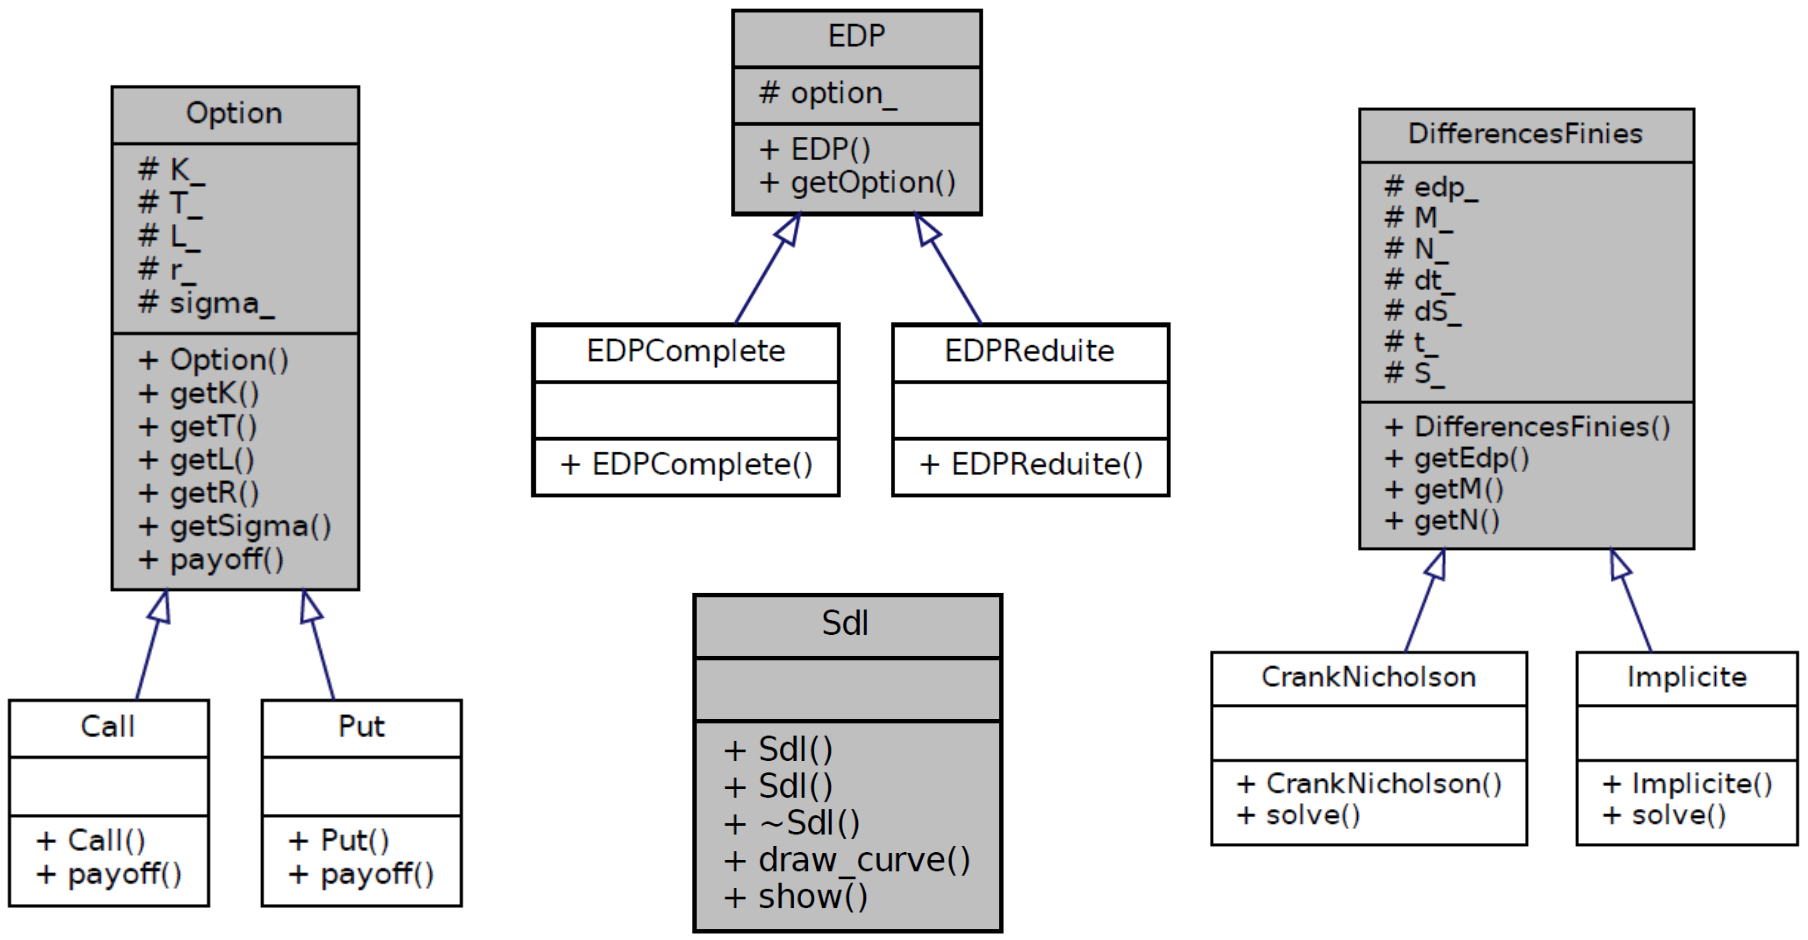
\includegraphics[scale=0.35]{UML.png}
    \caption{Diagramme des classes}
\end{figure}

\vspace{0.5cm}

\subsection{Diagramme des inclusions}

\begin{figure}[!ht]
    \centering
    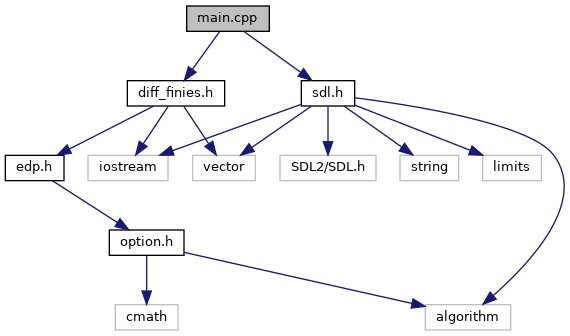
\includegraphics[scale=0.7]{include_graph.png}
    \caption{Diagramme des inclusions}
\end{figure}

\end{document}
